\documentclass[float=true,preview,class=scrartcl]{standalone}
\usepackage{tikz}
\usepackage{graphicx}
\usetikzlibrary{positioning}
\usetikzlibrary{calc}
\def\mainpath{../../}
\def\tikzpath{./}
\def\datapath{/home/lukas/Desktop/SA_Thesis/studies/2016-08-18_EigenvalueDistribution/output/sim}

\usepackage{import}
%\usepackage{subfigure}
\usepackage{subcaption}
\usepackage{capt-of}

\usepackage[outline]{contour}

\usepackage{pgfplots}
\usepackage{pgfplotstable}



\definecolor{list1_1}{RGB}{0,101,189}
\definecolor{list1_2}{RGB}{156,157,159}
\definecolor{list1_3}{RGB}{162,173,0}
\definecolor{list1_4}{RGB}{227,114,34} 
\definecolor{list1_5}{RGB}{152,198,234}


%\definecolor{list1_1}{RGB}{246,81,29}
%\definecolor{list1_2}{RGB}{255,180,0}
%\definecolor{list1_3}{RGB}{0,166,237}
%\definecolor{list1_4}{RGB}{127,184,0}
%\definecolor{list1_5}{RGB}{13,44,84}


\pgfplotscreateplotcyclelist{markerlist}{
list1_1, thick, solid, mark=*\\%
list1_2, thick, solid, mark=asterisk\\%
list1_3, thick, solid, mark=diamond*\\%
list1_4, thick, solid, mark=triangle\\%
list1_5, thick, solid, mark=square\\%
}

\pgfplotscreateplotcyclelist{linelist}{
list1_1, solid\\%
list1_2, solid\\%
list1_3, solid\\%
list1_4, solid\\%
list1_5, solid\\%
}

\definecolor{lightgrey}{RGB}{200,200,200}
\definecolor{nassitextcolor}{RGB}{0,0,200}
\begin{document}


%\begin{figure}[htb]
%    \begin{subfigure}[b]{0.8\textwidth}
%        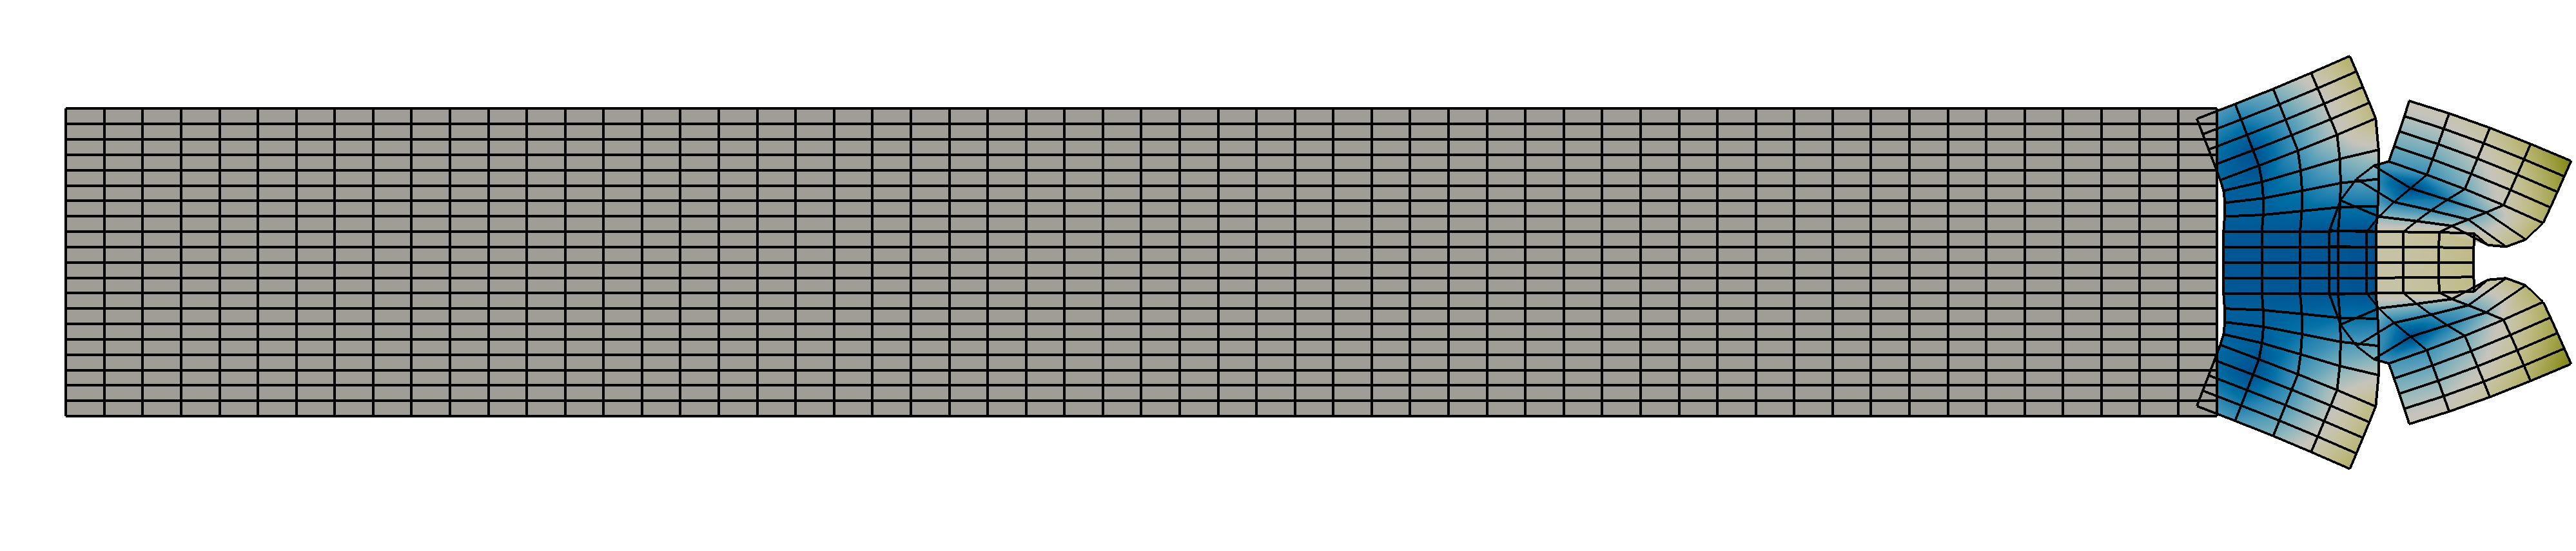
\includegraphics[width=\textwidth]{/home/lukas/Desktop/SA_Thesis/studies/2016-08-18_EigenvalueDistribution/setup/feti1_iter1.pdf}
%        \caption{iteration 1}
%    \end{subfigure}
%    \vskip\baselineskip
%    \begin{subfigure}[b]{0.8\textwidth}
%        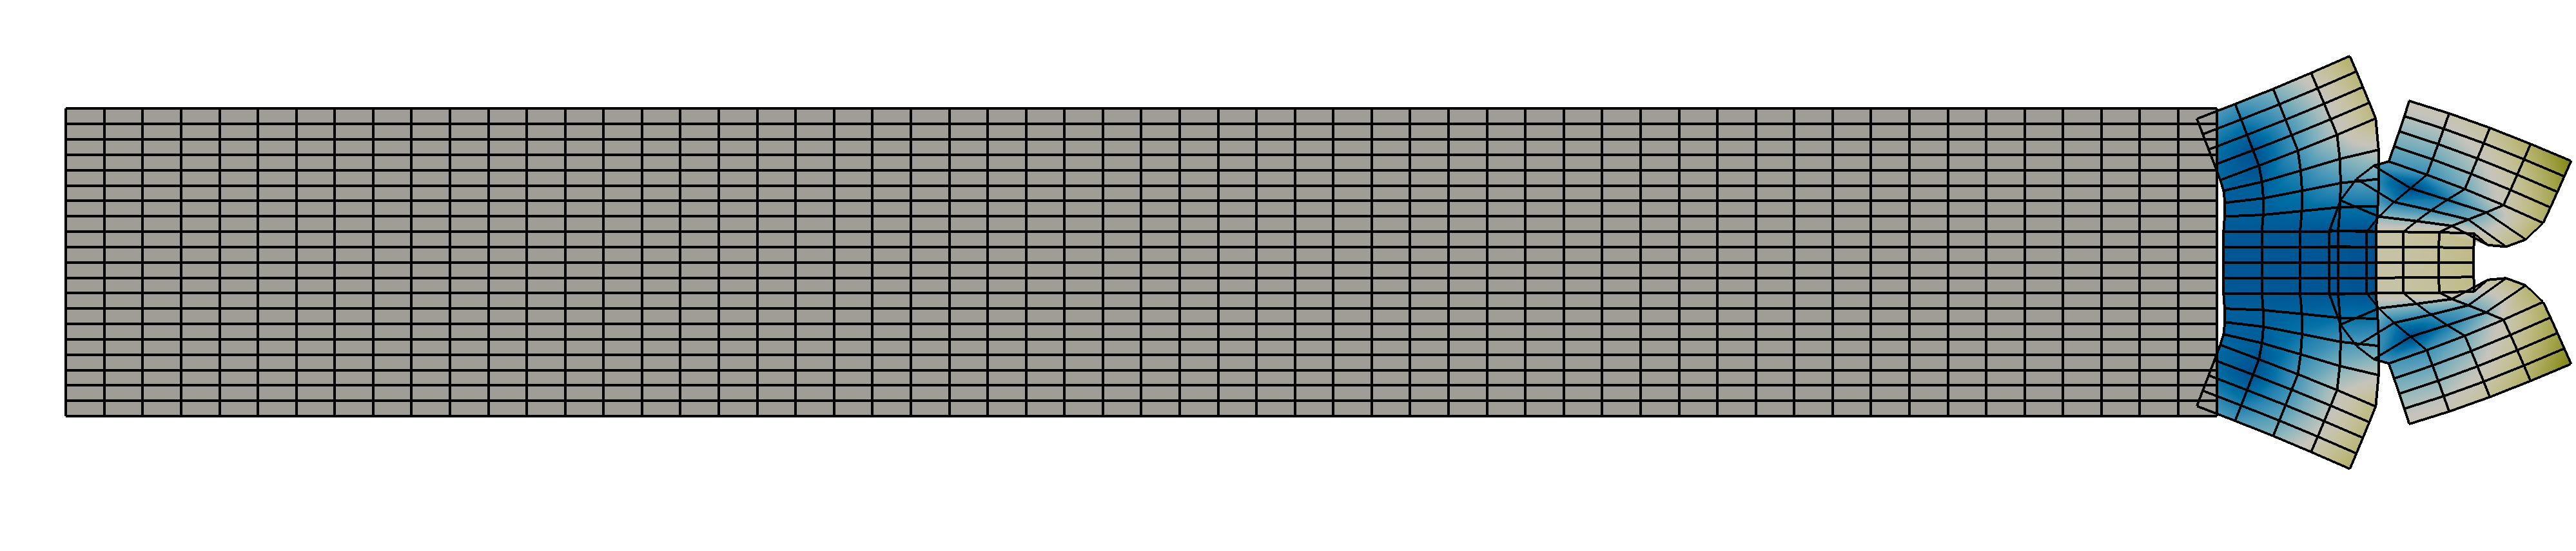
\includegraphics[width=\textwidth]{/home/lukas/Desktop/SA_Thesis/studies/2016-08-18_EigenvalueDistribution/setup/feti1_iter1.pdf}
%        \caption{iteration 2}
%    \end{subfigure}
%    \vskip\baselineskip
%    \begin{subfigure}[b]{0.8\textwidth}
%        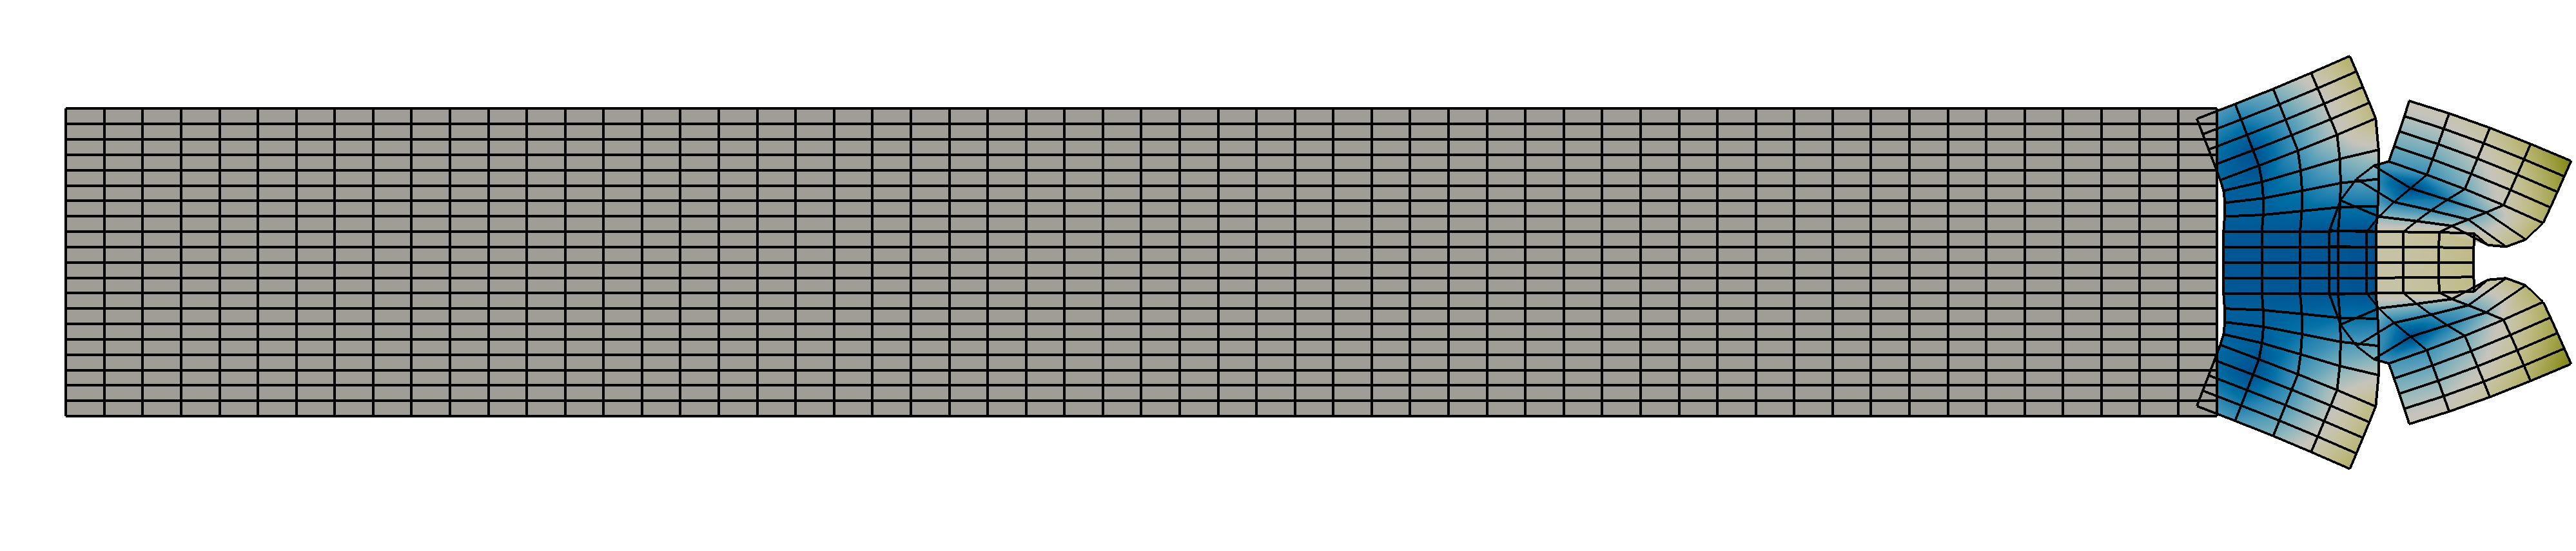
\includegraphics[width=\textwidth]{/home/lukas/Desktop/SA_Thesis/studies/2016-08-18_EigenvalueDistribution/setup/feti1_iter1.pdf}
%        \caption{iteration 3}
%    \end{subfigure}
%    \vskip\baselineskip
%    \begin{subfigure}[b]{0.8\textwidth}
%        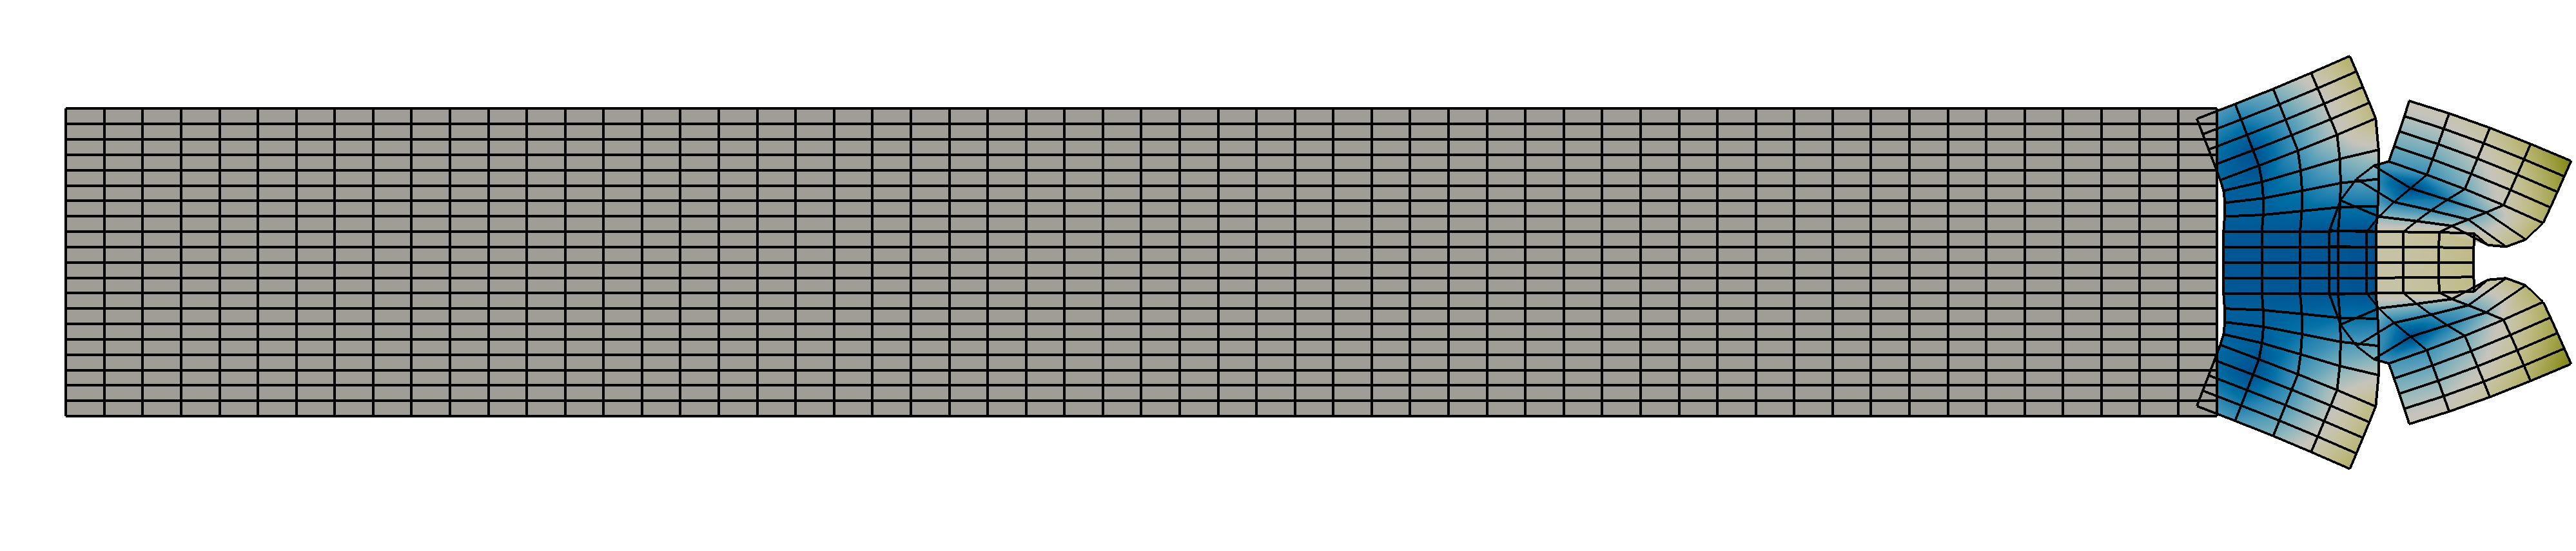
\includegraphics[width=\textwidth]{/home/lukas/Desktop/SA_Thesis/studies/2016-08-18_EigenvalueDistribution/setup/feti1_iter1.pdf}
%        \caption{final iteration}
%    \end{subfigure}
%\end{figure} 



\begin{tikzpicture}
\def\ydist{-2.1}
\node[inner sep=0pt] (russell) at (0,0)
    {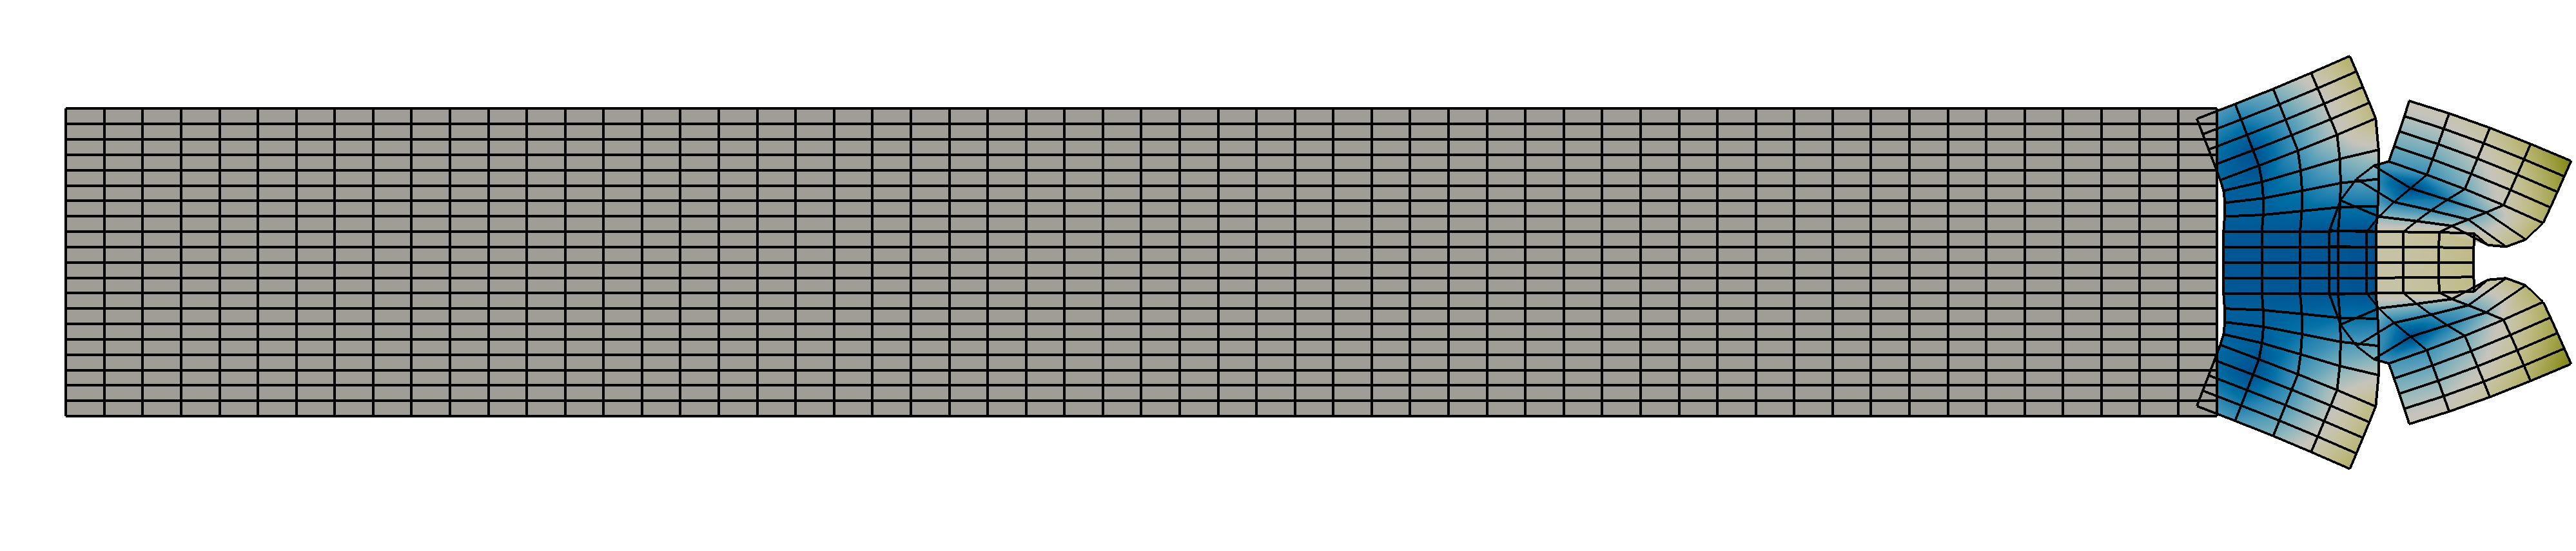
\includegraphics[width=.7\textwidth]{/home/lukas/Desktop/SA_Thesis/studies/2016-08-18_EigenvalueDistribution/setup/feti1_iter1.pdf}};
\node at (-5.5,0) [anchor=north west, scale=0.7, black, fill=white] {iteration 1}; 
    
\node[inner sep=0pt] (russell) at (0,\ydist)
    {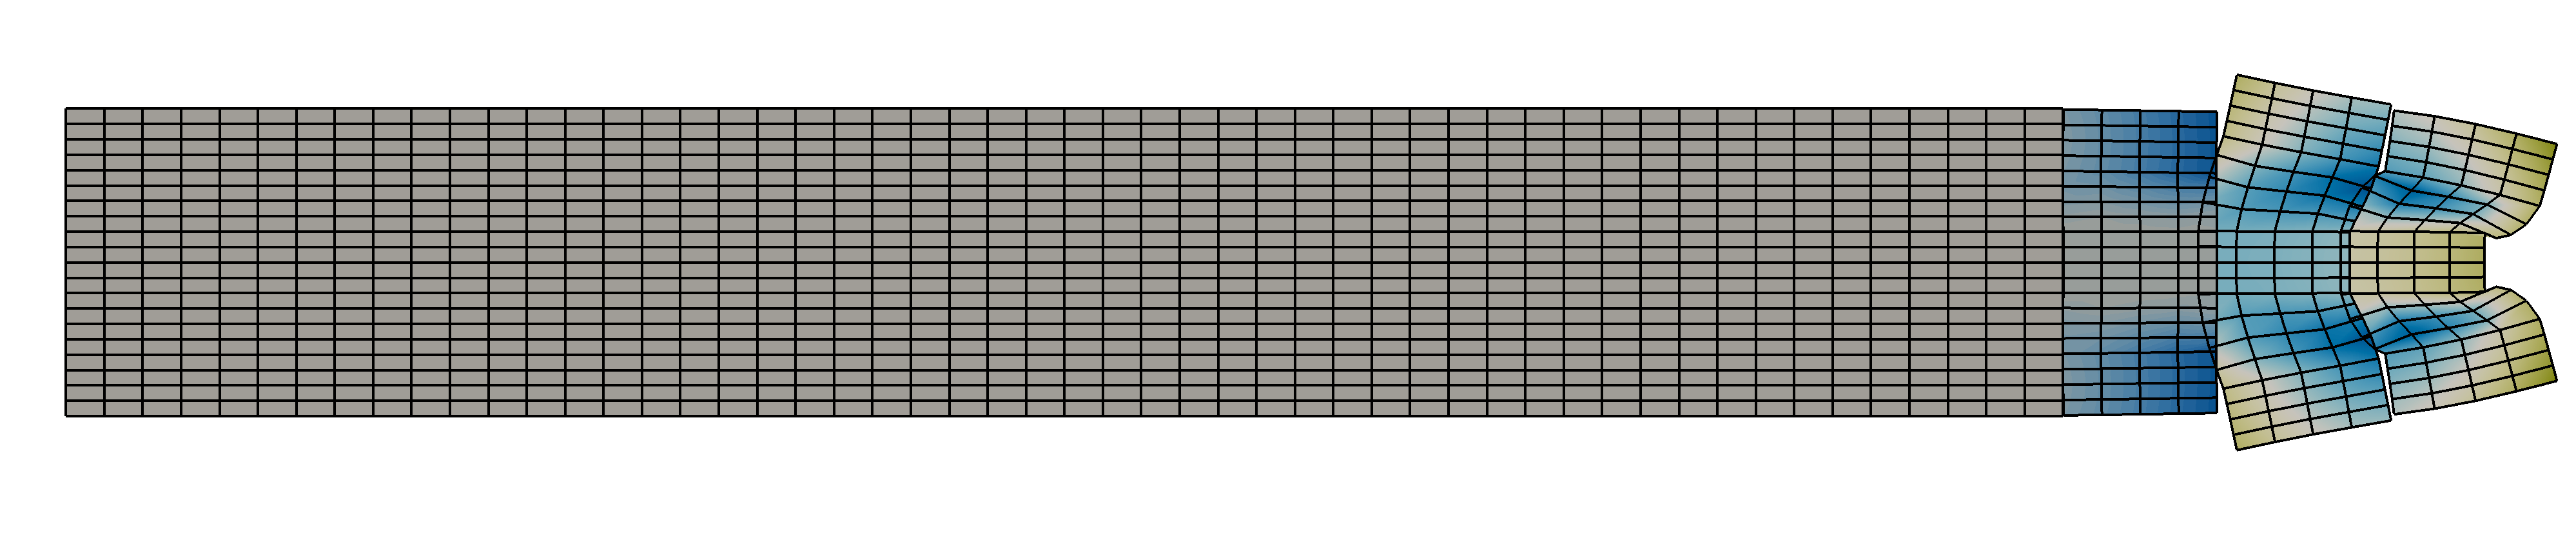
\includegraphics[width=.7\textwidth]{/home/lukas/Desktop/SA_Thesis/studies/2016-08-18_EigenvalueDistribution/setup/feti1_iter2.pdf}};
\node at (-5.5,\ydist) [anchor=north west, scale=0.7, black, fill=white] {iteration 2}; 
    
\node[inner sep=0pt] (russell) at (0,2*\ydist)
    {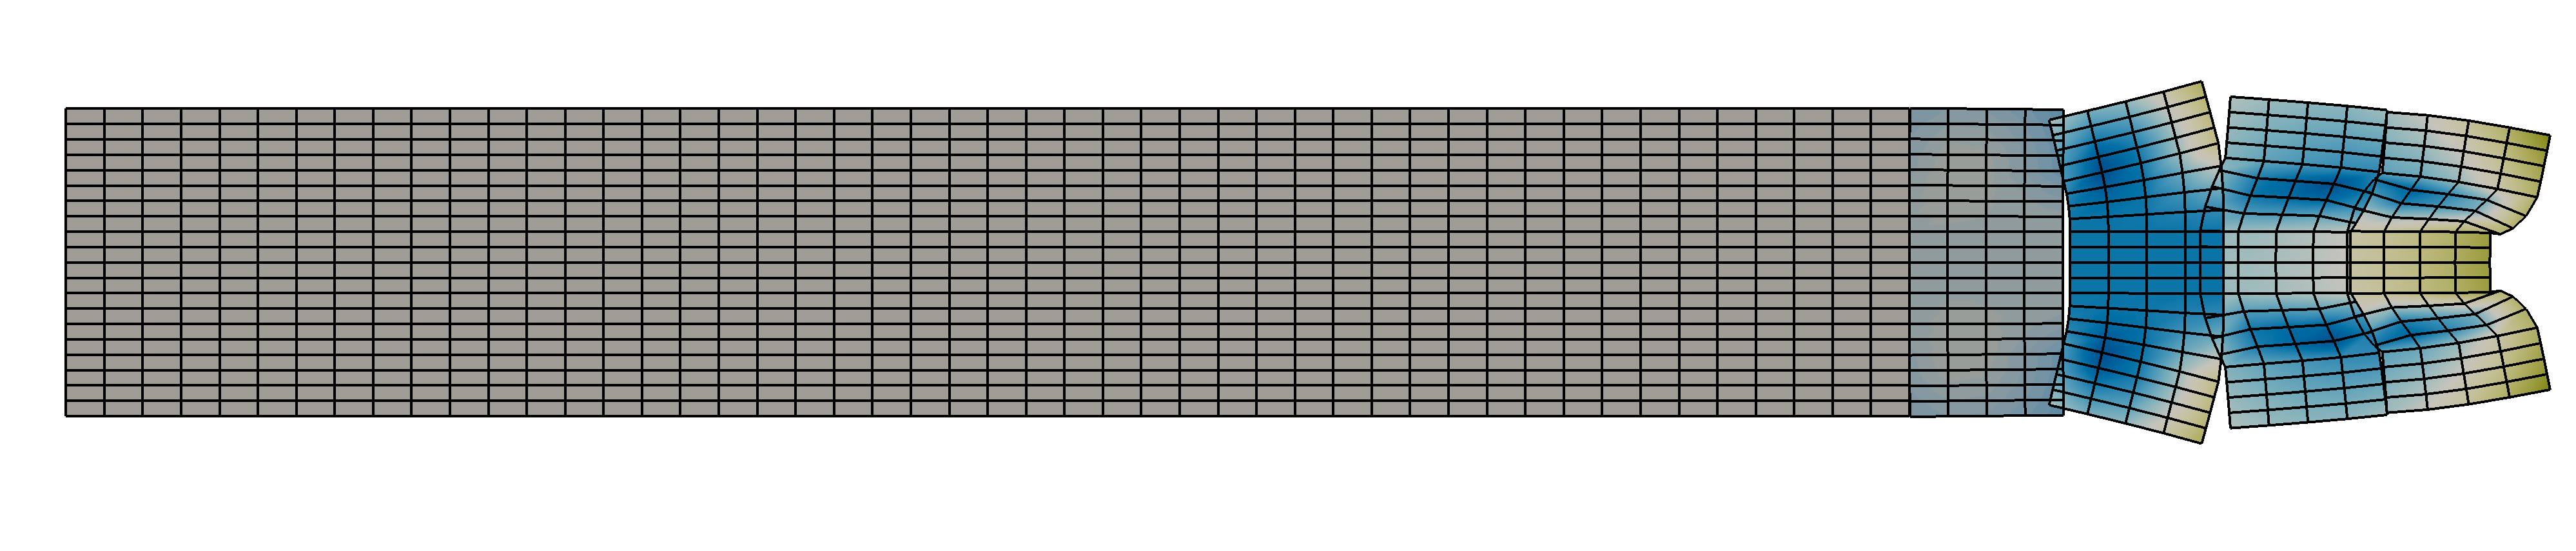
\includegraphics[width=.7\textwidth]{/home/lukas/Desktop/SA_Thesis/studies/2016-08-18_EigenvalueDistribution/setup/feti1_iter3.pdf}};
\node at (-5.5,2*\ydist) [anchor=north west, scale=0.7, black, fill=white] {iteration 3}; 
    
\node[inner sep=0pt] (russell) at (0,3*\ydist)
    {\includegraphics[width=.7\textwidth]{/home/lukas/Desktop/SA_Thesis/studies/2016-08-18_EigenvalueDistribution/setup/feti1_iterfinal.pdf}};
\node at (-5.5,3*\ydist) [anchor=north west, scale=0.7, black, fill=white] {converged}; 
    
    \node[inner sep=0pt] (russell) at (0,3.6*\ydist)
{
\includegraphics[width=.7\textwidth]{/home/lukas/Desktop/SA_Thesis/studies/2016-08-18_EigenvalueDistribution/setup/feti1_iter_colormap.pdf}};
\end{tikzpicture}



\end{document}